\section{fireMIP}
\pgfdeclareimage[width=1.0\paperwidth]{header-image}{header_images/red_lightn}

\begin{frame}<3-4>[label = fireModels]
	\frametitle{fire Models}
	\framesubtitle{Types}
	\foreach \x in {1, 2, 3, 4} {
		\only<\x> {
			\includegraphics[width=10cm]{images/fireModelTypes/pp\x.png}
	}}	
\end{frame}

%\addtocounter{framenumber}{-1}
\pgfdeclareimage[width=1.0\paperwidth]{header-image}{header_images/kata_tjuta}

\begin{frame}[label = kelley2013Datasets]
	\frametitle{FireMIP benchmarking}
	\framesubtitle{Benchmark Datasets}
	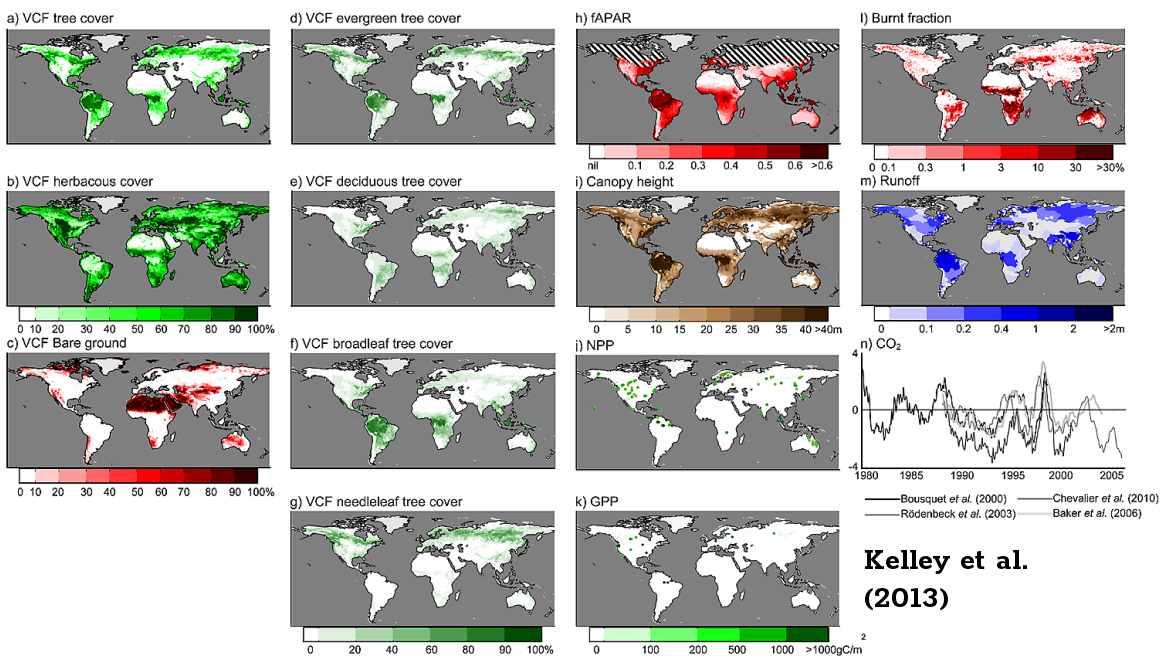
\includegraphics[width=11.5cm]{images/BenchmarkDatasets.png}
	\visible<1-2> {
		\begin{center}
			Plus some new ones
		\end{center}
	}
\end{frame}

\addtocounter{framenumber}{-1}

\begin{frame}[label = newDatasets]
	\frametitle{FireMIP benchmarking}
	\framesubtitle{Fire Benchmark Datasets}
	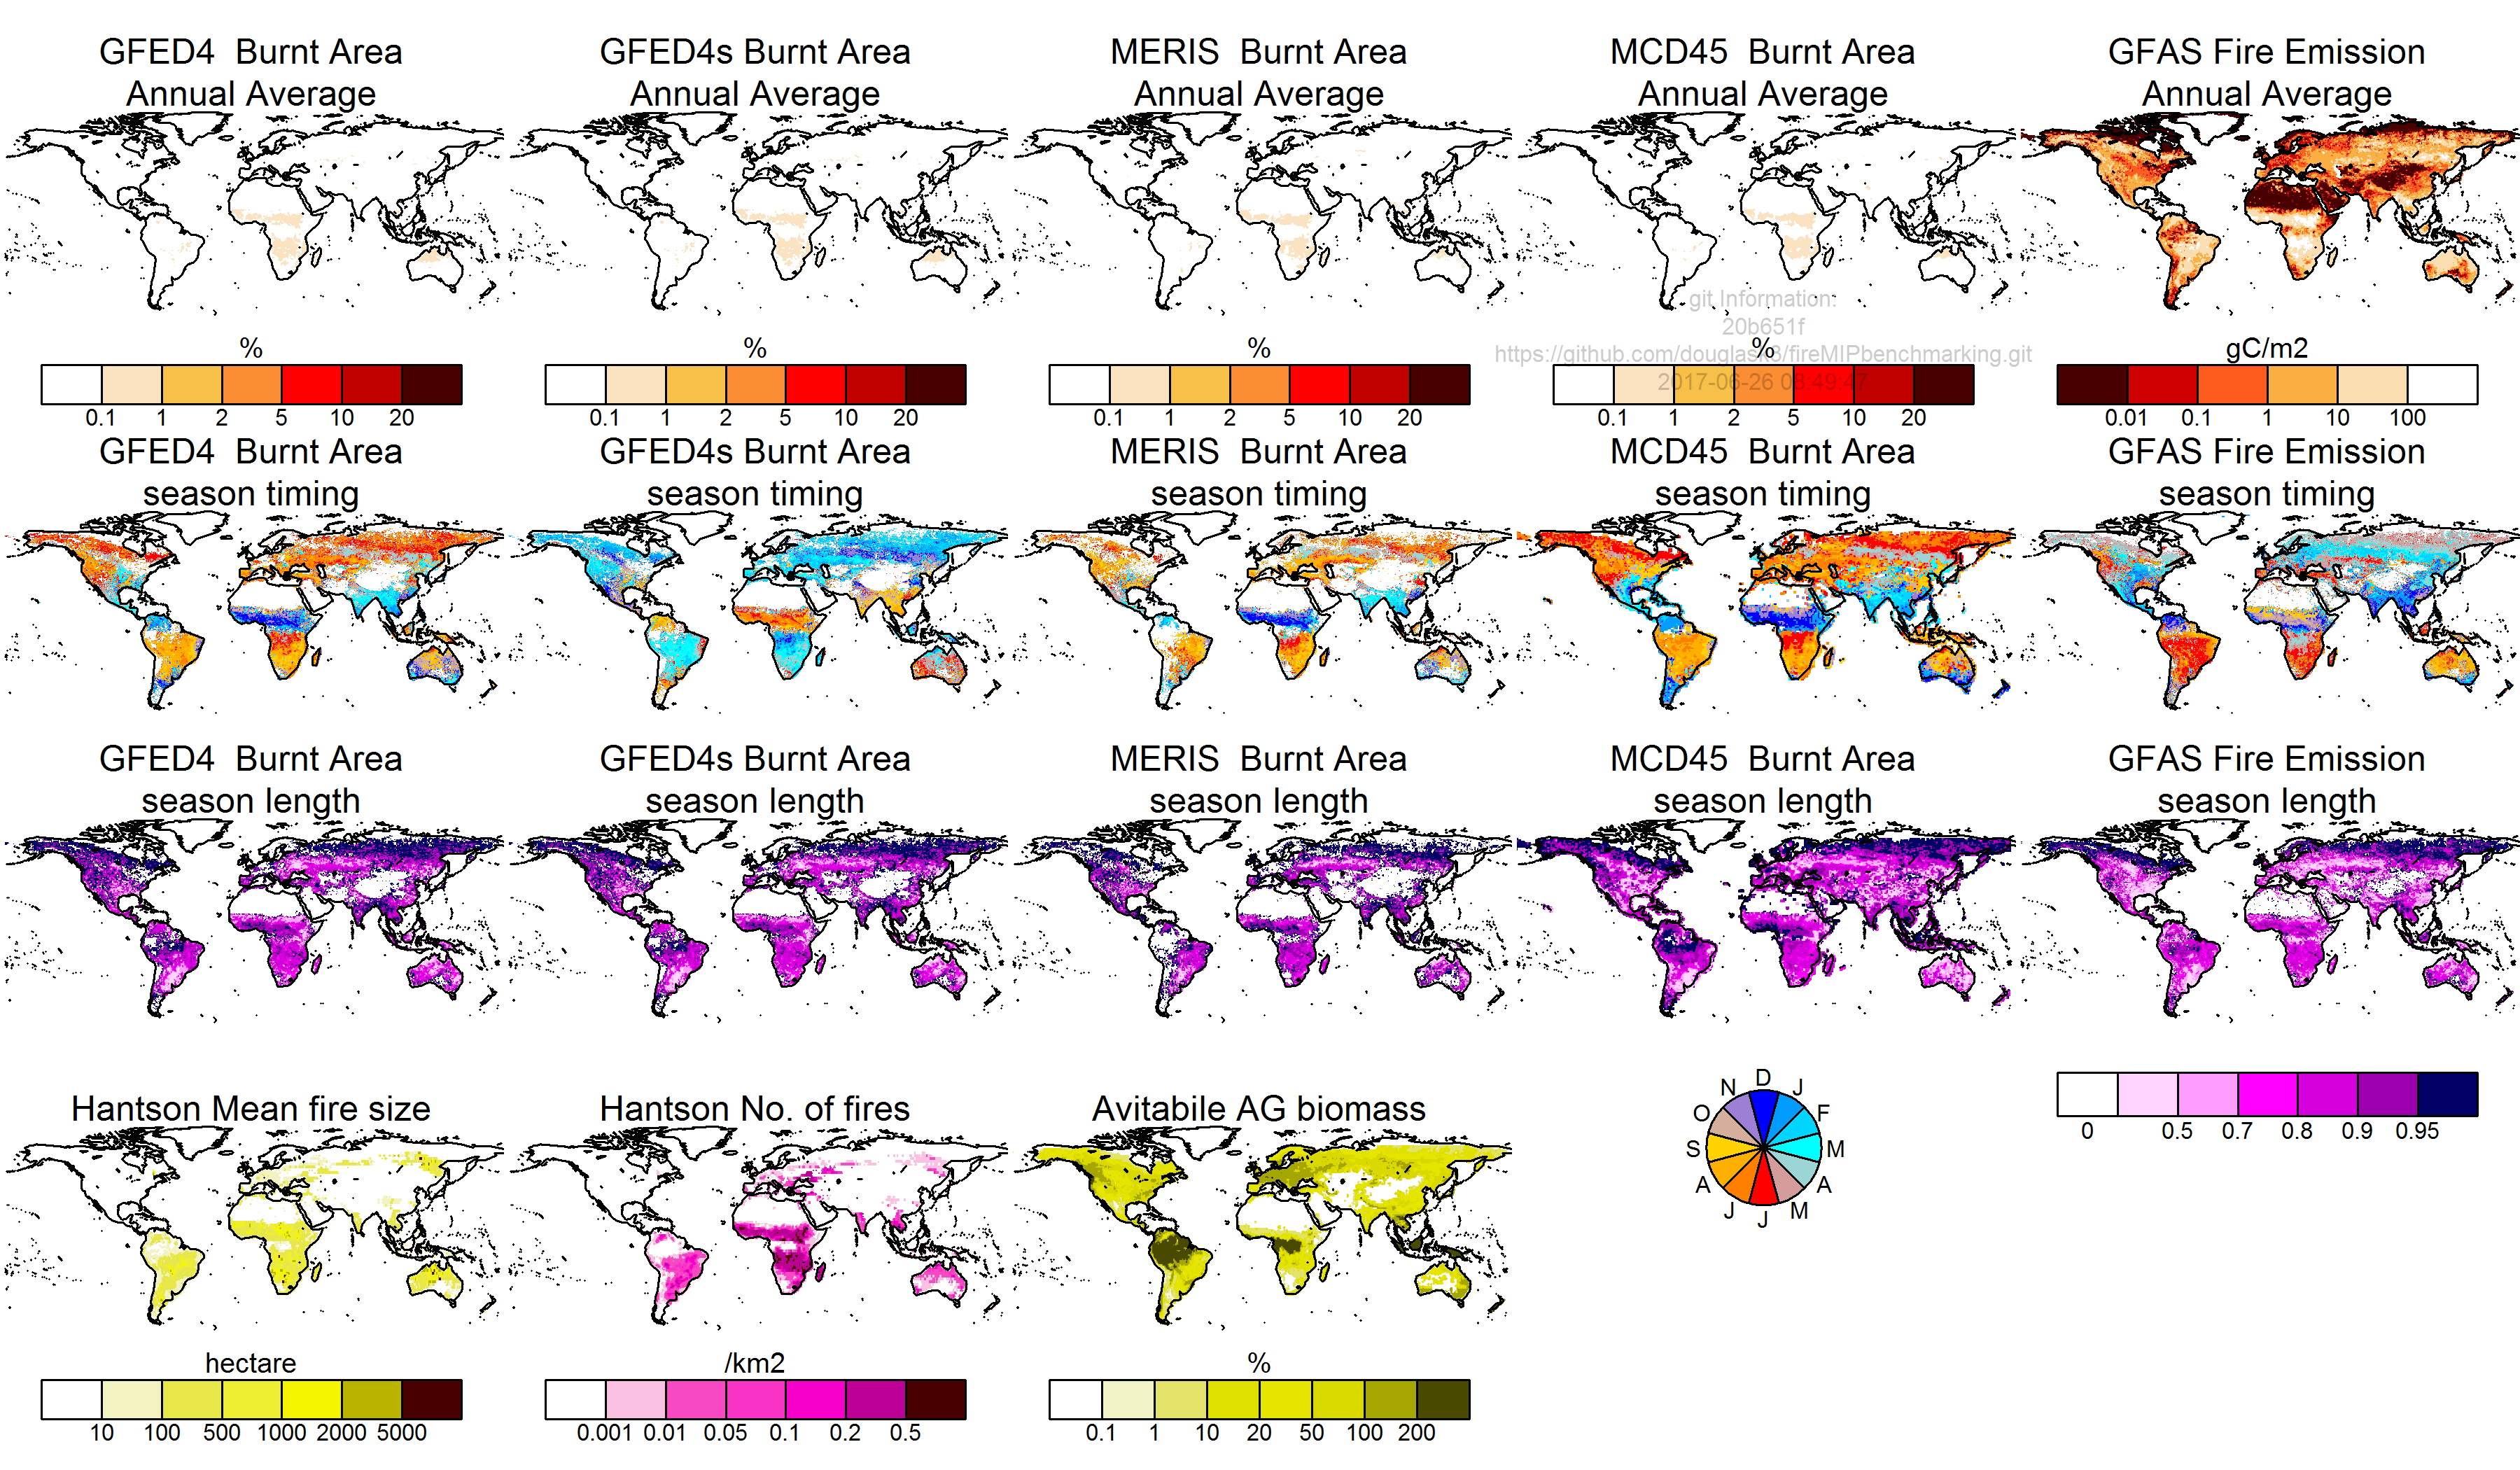
\includegraphics[width=11.5cm]{../../figs/burntAreaProducts.png}
\end{frame}

\begin{frame}<1,1>[label = Metrics]
	\frametitle{FireMIP Metrics}
	\framesubtitle{All Metrics}
	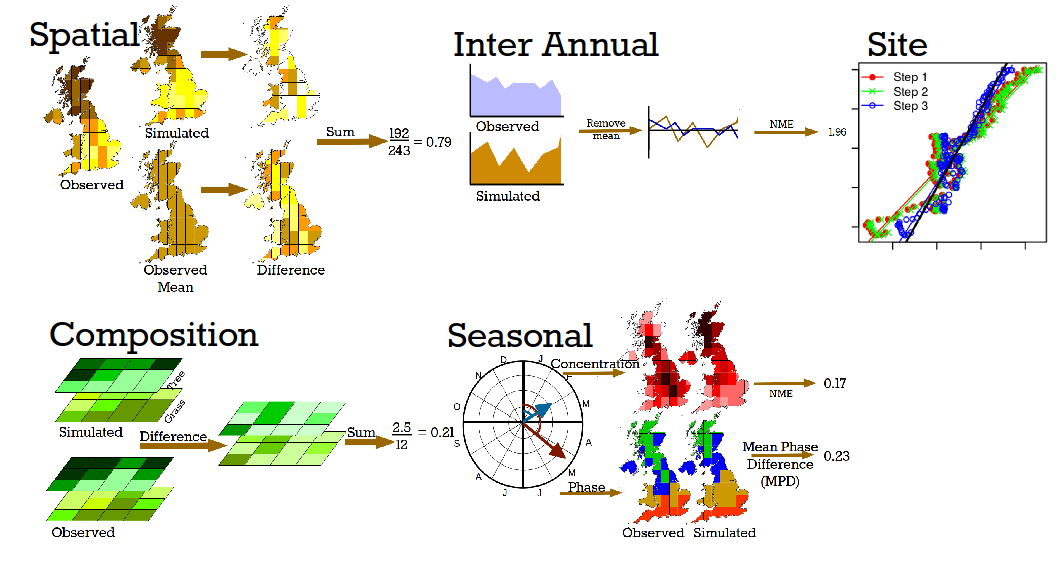
\includegraphics[width=11.5cm]{images/metrics/Metrics.png}
\end{frame}

\addtocounter{framenumber}{-1}

\begin{frame}<4>[label = MetricsNME]
	\frametitle{FireMIP Metrics}
	\framesubtitle{Normalised Mean Error}
	\foreach \x in {1, 2, 3, 4} {
		\only<\x> {
			\includegraphics[width=10cm]{images/metrics/NME/NME\x.png}
	}}
\end{frame}

\addtocounter{framenumber}{-1}

\begin{frame}<2->[label = MetricsMPD]
	\frametitle{FireMIP Metrics}
	\framesubtitle{Seasonal Comparisons}
	\foreach \x in {1, 2, 3, 4, 5, 6, 7} {
		\only<\x> {
			\includegraphics[width=10cm]{images/metrics/MPD/MPD\x.png}
	}}
\end{frame}

\addtocounter{framenumber}{-1}

\begin{frame}<4>[label = NullModels]
	\frametitle{FireMIP Null Models}
	%\framesubtitle{Seasonal Comparisons}
	\foreach \x in {1,2,3,4} {
		\only<\x> {
			\includegraphics[width=10cm]{images/metrics/NULL/NullModels\x.png}
	}}
\end{frame}

\addtocounter{framenumber}{-1}

\begin{frame}<1-2>[label = Scores]
	\frametitle{FireMIP Null Models}
	%\framesubtitle{Seasonal Comparisons}
	\foreach \x in {1, 2, 3} {
		\only<\x> {
			\includegraphics[width=10cm]{images/metrics/Scores/Scores\x.png}
	}}
\end{frame}